% !TeX root = proposal.tex
\section{Hypervisor-mediated API-remoting}
\label{sec:ava}

Practical virtualization must support sharing and isolation under flexible
policy with minimal overhead. The structure of current accelerator stacks
makes this extremely difficult to achieve.
Accelerator stacks are \emph{silos} (Figure~\ref{fig:silo})
comprising proprietary layers communicating through memory mapped interfaces.
This opaque organization makes it \emph{impossible} to interpose intermediate
layers cleanly to form a virtualization boundary. Practically interposable
alternatives leave designers with a Hobson's choice between critical
virtualization properties such as interposition and compatibility.

\begin{figure}[!ht]
	\centering
	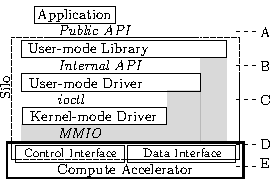
\includegraphics[width=.4\linewidth]{figures/silo.pdf}
	\caption{An accelerator silo.
		The public API and the interfaces with striped backgrounds are interposition candidates.
		All interfaces with backgrounds are proprietary and subject to change.
        }
	\label{fig:silo}
\end{figure}

We present \textsc{AvA}, a system that addresses the fundamental limitations
of existing accelerator virtualization techniques.
\textsc{AvA} combines API-agnostic para-virtual I/O stack components with a
Domain-Specific Language (DSL) and toolchain to automate construction
and deployment of guest libraries and API servers.
\textsc{AvA} uses an abstract para-virtual device to serve as a transport
endpoint for forwarding the public APIs of vendor-provided frameworks (e.g.
CUDA or TensorFlow). Unlike currently popular user-space API remoting
solutions~\cite{bitfusion,xaas,vmCUDA,rCUDA,cu2rcu}, \textsc{AvA} preserves
hypervisor-level resource management and strong isolation using a novel
technique called \emph{{{H}ypervisor {I}nterposed {R}emote {A}cceleration}}.
\textsc{AvA} forwards API calls over hypervisor-managed communication channels,
inserting automatically-generated resource management components between
traditional front- and back-ends
to enforce policies described in the DSL specification.
Critically, \emph{automation} from \textsc{AvA} enables hypervisors to keep up
with fast accelerator evolution: automatic generation of components minimizes
engineering effort.

\textsc{AvA} supports a broad range of currently-shipping compute accelerators:
We virtualized ten accelerators including NVIDIA and AMD GPUs, Google TPUs,
and Intel QuickAssist.
Virtualizing an API framework using \textsc{AvA} requires modest developer
effort:
a single developer virtualized OpenCL in a handful of days,
a stark contrast to the person-years of developer effort for VMware's SVGA II
or Bitfusion's FlexDirect~\cite{bitfusion}.
Experiments show that \textsc{AvA} provides near-native performance (e.g., 2.4\% slowdown for TensorFlow and 5.6\% for CUDA), enforces isolation and fair sharing across guests, and supports live migration.

The proposed chapter will make the following arguments:

\begin{itemize}[nosep,leftmargin=1em,labelwidth=*,align=left]
\item The chapter demonstrates feasibility of automatically constructed virtual accelerator support, showing that a single technique can deal with many architectures, APIs, versions, and policies.
\item We introduce {{H}ypervisor {I}nterposed {R}emote {A}cceleration} (HIRA) to enable hypervisor-enforced isolation and sharing policies unachievable with current SR-IOV and API remoting systems.
\item We utilize a novel DSL, \textsc{Lapis}, for describing API functions, resources, and policies to enable automatic construction of virtual stacks from native header files.
\item Our evaluation shows low developer effort, strong isolation, and good performance.
\end{itemize}

This chapter will draw from joint work with Hangchen Yu, Arthur Peters and
Christopher J Rossbach. Part of this work was published as a workshop
paper~\cite{ava-hotos}, and a longer paper is under submission. As with any
big system building effort, it was a team effort. This material will be a part
of Hangchen's and Arthur's dissertations as well, and we have agreed to split
the intellectual contributions from the project thus: While I will focus on
the core virtualization technique, i.e, hypervisor-mediated API-remoting in my
dissertation, Hangchen's dissertation will deal with the challenges of
designing API-remoting systems for both virtualization as well as use from
within an OS kernel; Arthur's dissertation will focus on the specification and
design of LAPIS, a DSL for specifying and generating remoting code for
arbitrary C APIs.